
% Chapter Template
\setstretch{1}
\chapter{Hardware Deployment in Limited Local Space}\thispagestyle{empty} % Main chapter title

\label{Chapter4} 

\lhead{Chapter 4. \emph{Hardware Deployment in Limited Local Space}}
\setstretch{2}
\begin{figure}[!ht]
 \centering
  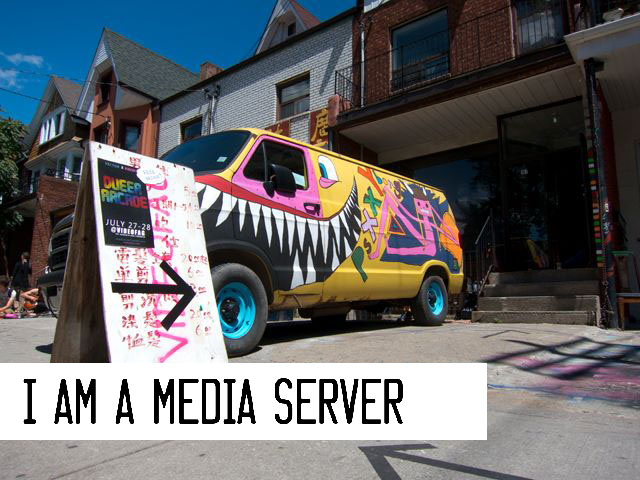
\includegraphics[width=\textwidth]{psXXYborgVan3}
  \caption{Hannah Epstein\\ psXXYborg at VideoFag, 1995}
\end{figure}

\begin{figure}[!ht]
 \centering
  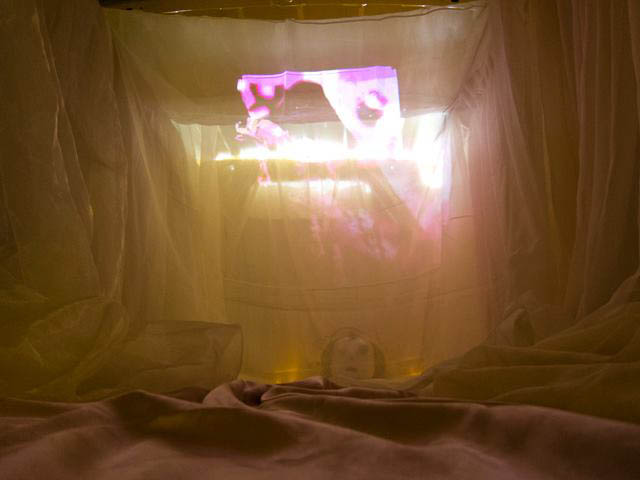
\includegraphics[width=\textwidth]{psXXYborgInterior}
  \caption{Hannah Epstein, Alex Leitch, Sagan Yee\\ psXXYborg at VideoFag, 1995}
\end{figure}
\newpage
\newpage

\section{Public Installations}
During the course of this project, games made with ScreenPerfect had many public outings. We installed psXXYborg specifically in a variety of spaces, and there were a number of design approaches to the construction of those spaces, governed mainly by Hannah Epstein. Hannah and I decided through a series of conversations on a number of designs for display spaces for psXXYborg, including a straight projection on mylar, a whole-room space that would encompass the user in different projected, linked screens, and ultimately a portable "confessional" booth. The first variant of this is displayed in Figure 4.1, a custom-painted cargo van which we displayed at Videofag in Kensington Market as part of the Queer Arcade with Vector Art|Game Festival as part of their 2013 show (\url{http://www.vectorfestival.org/}).

More recent exhibitions of psXXYborg have been built into a tent, which can be more easily displayed indoors. The psXXYborg tent has been exhibited at Long Winter in December 2013 and at the Feminist Art Collective's annual conference at OCADu in 2014 (Figure 4.3, 4.4).

\newpage
\begin{figure}[!ht]
 \centering
  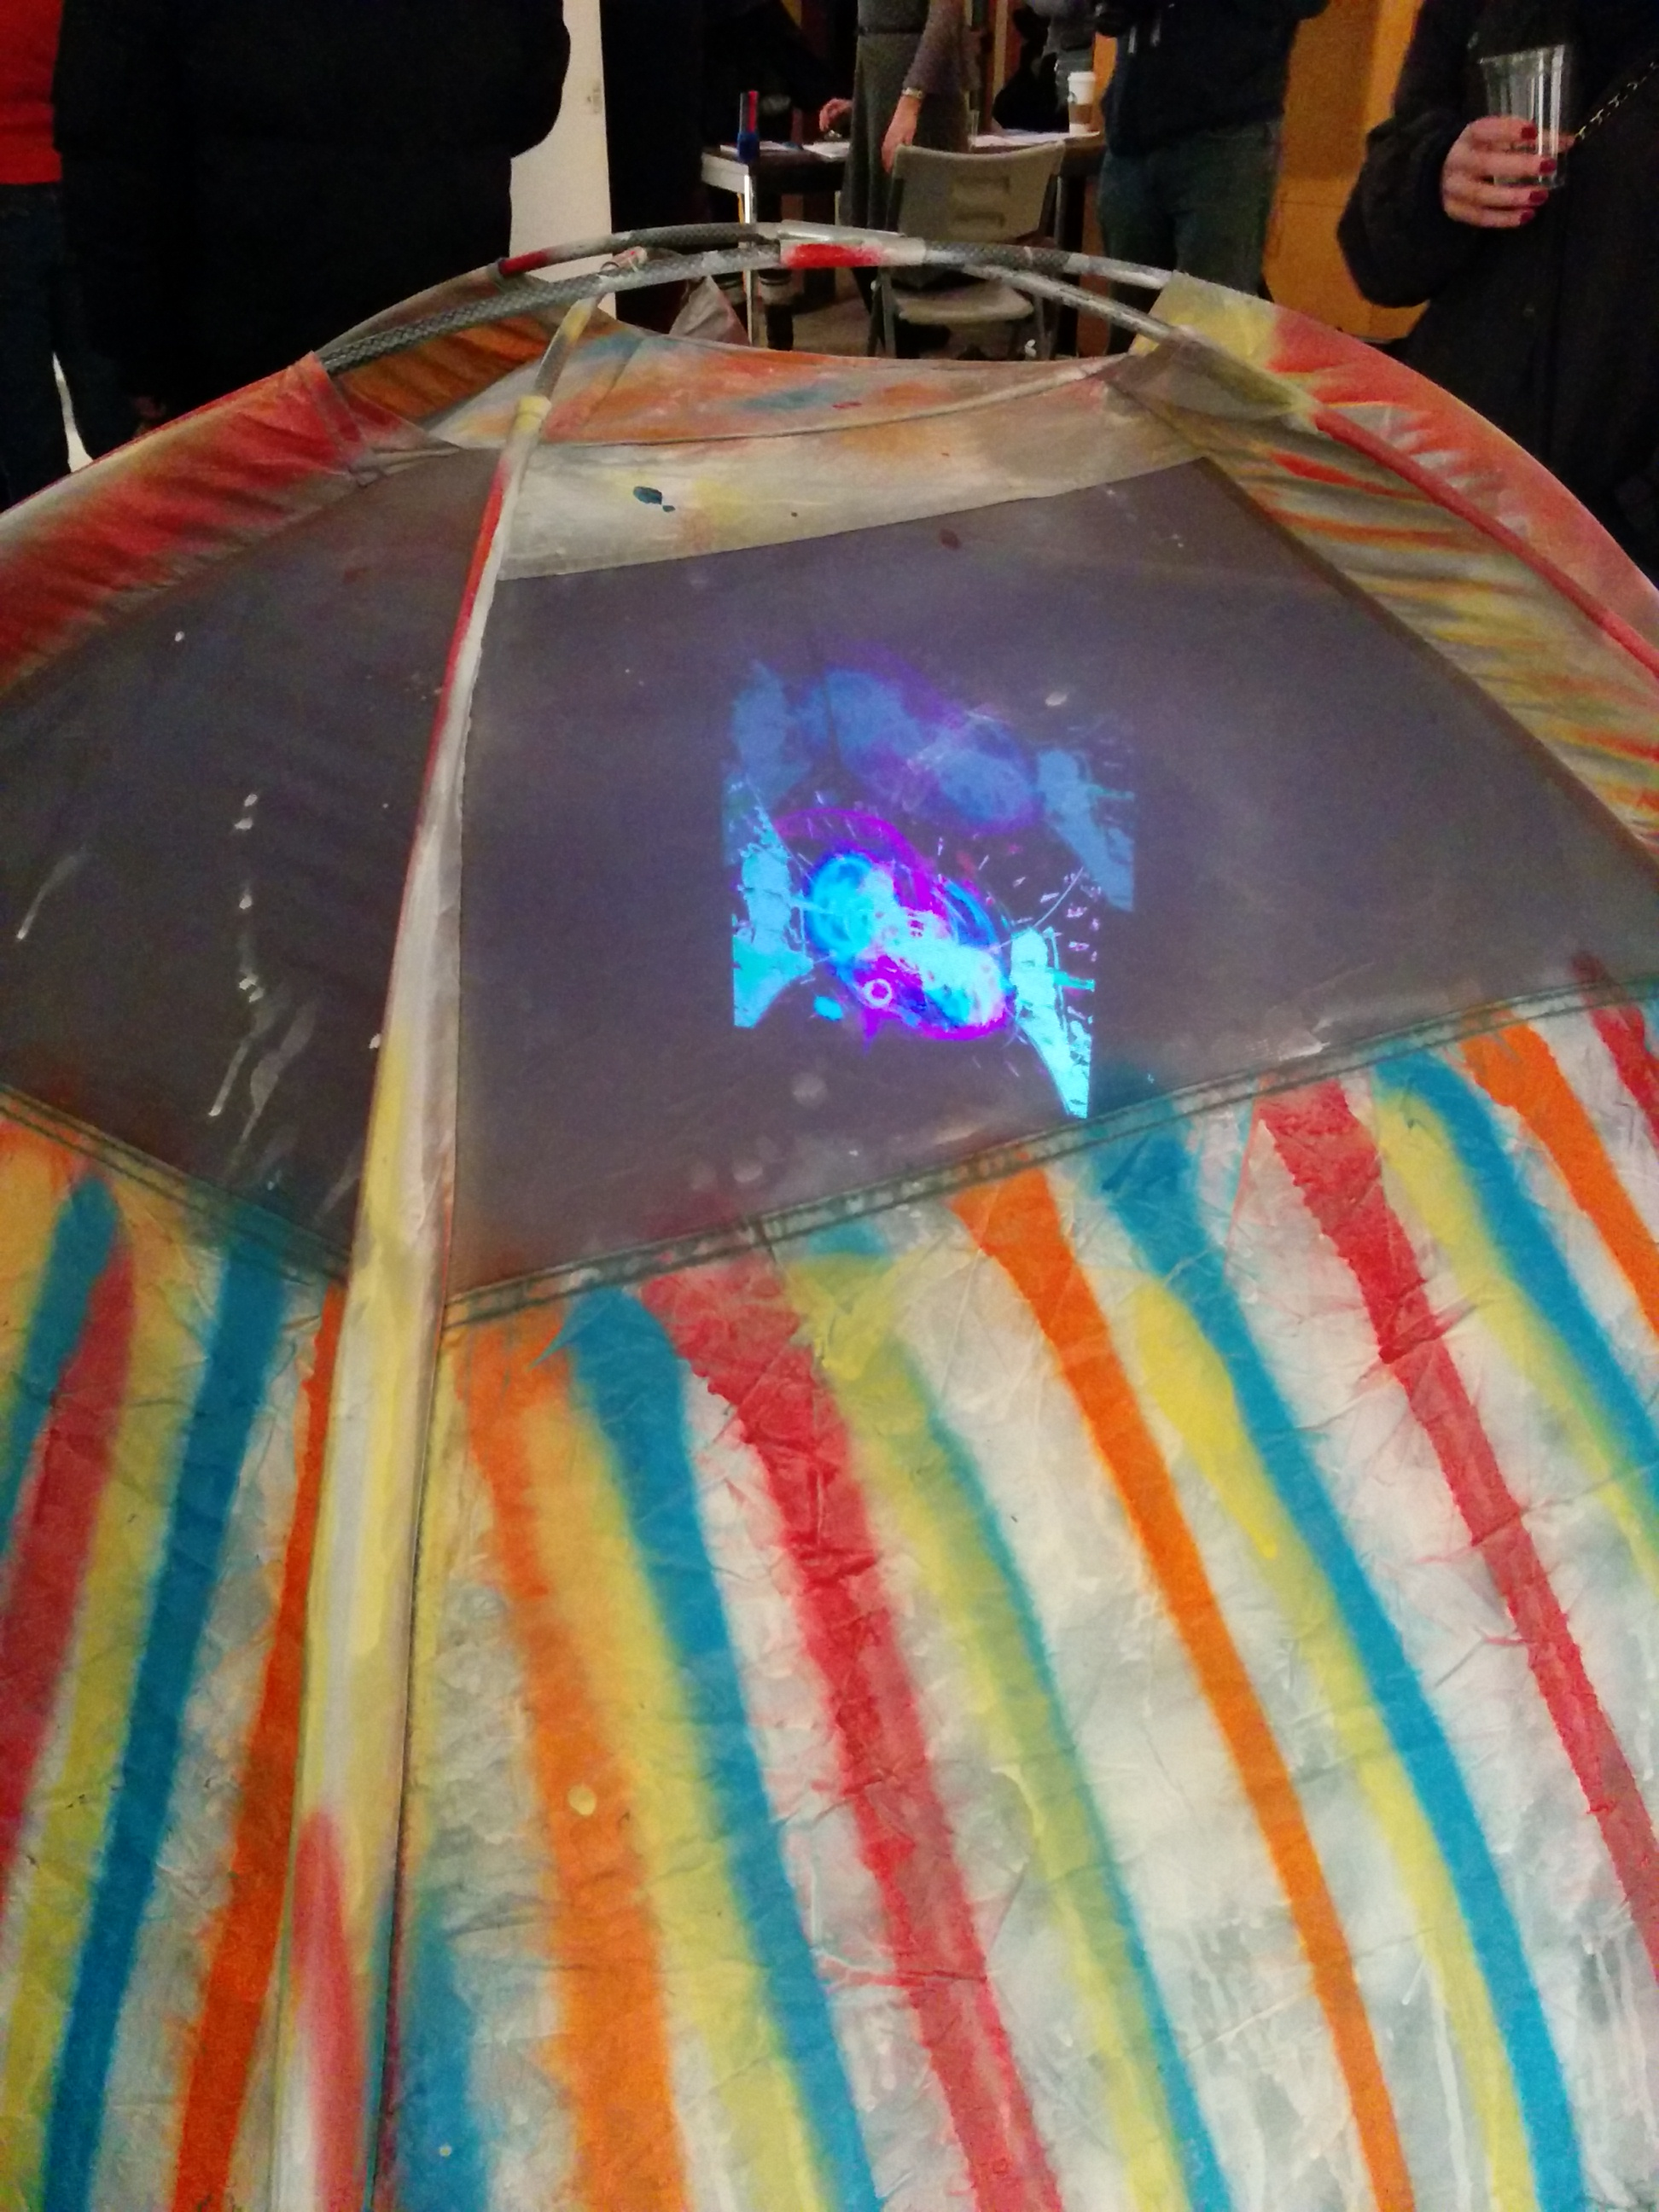
\includegraphics[width=0.7\textwidth]{psXXYborgTent}
  \caption{Hannah Epstein\\psXXYborg at FAC 2014}
\end{figure}

\clearpage
\begin{figure}[!ht]
 \centering
  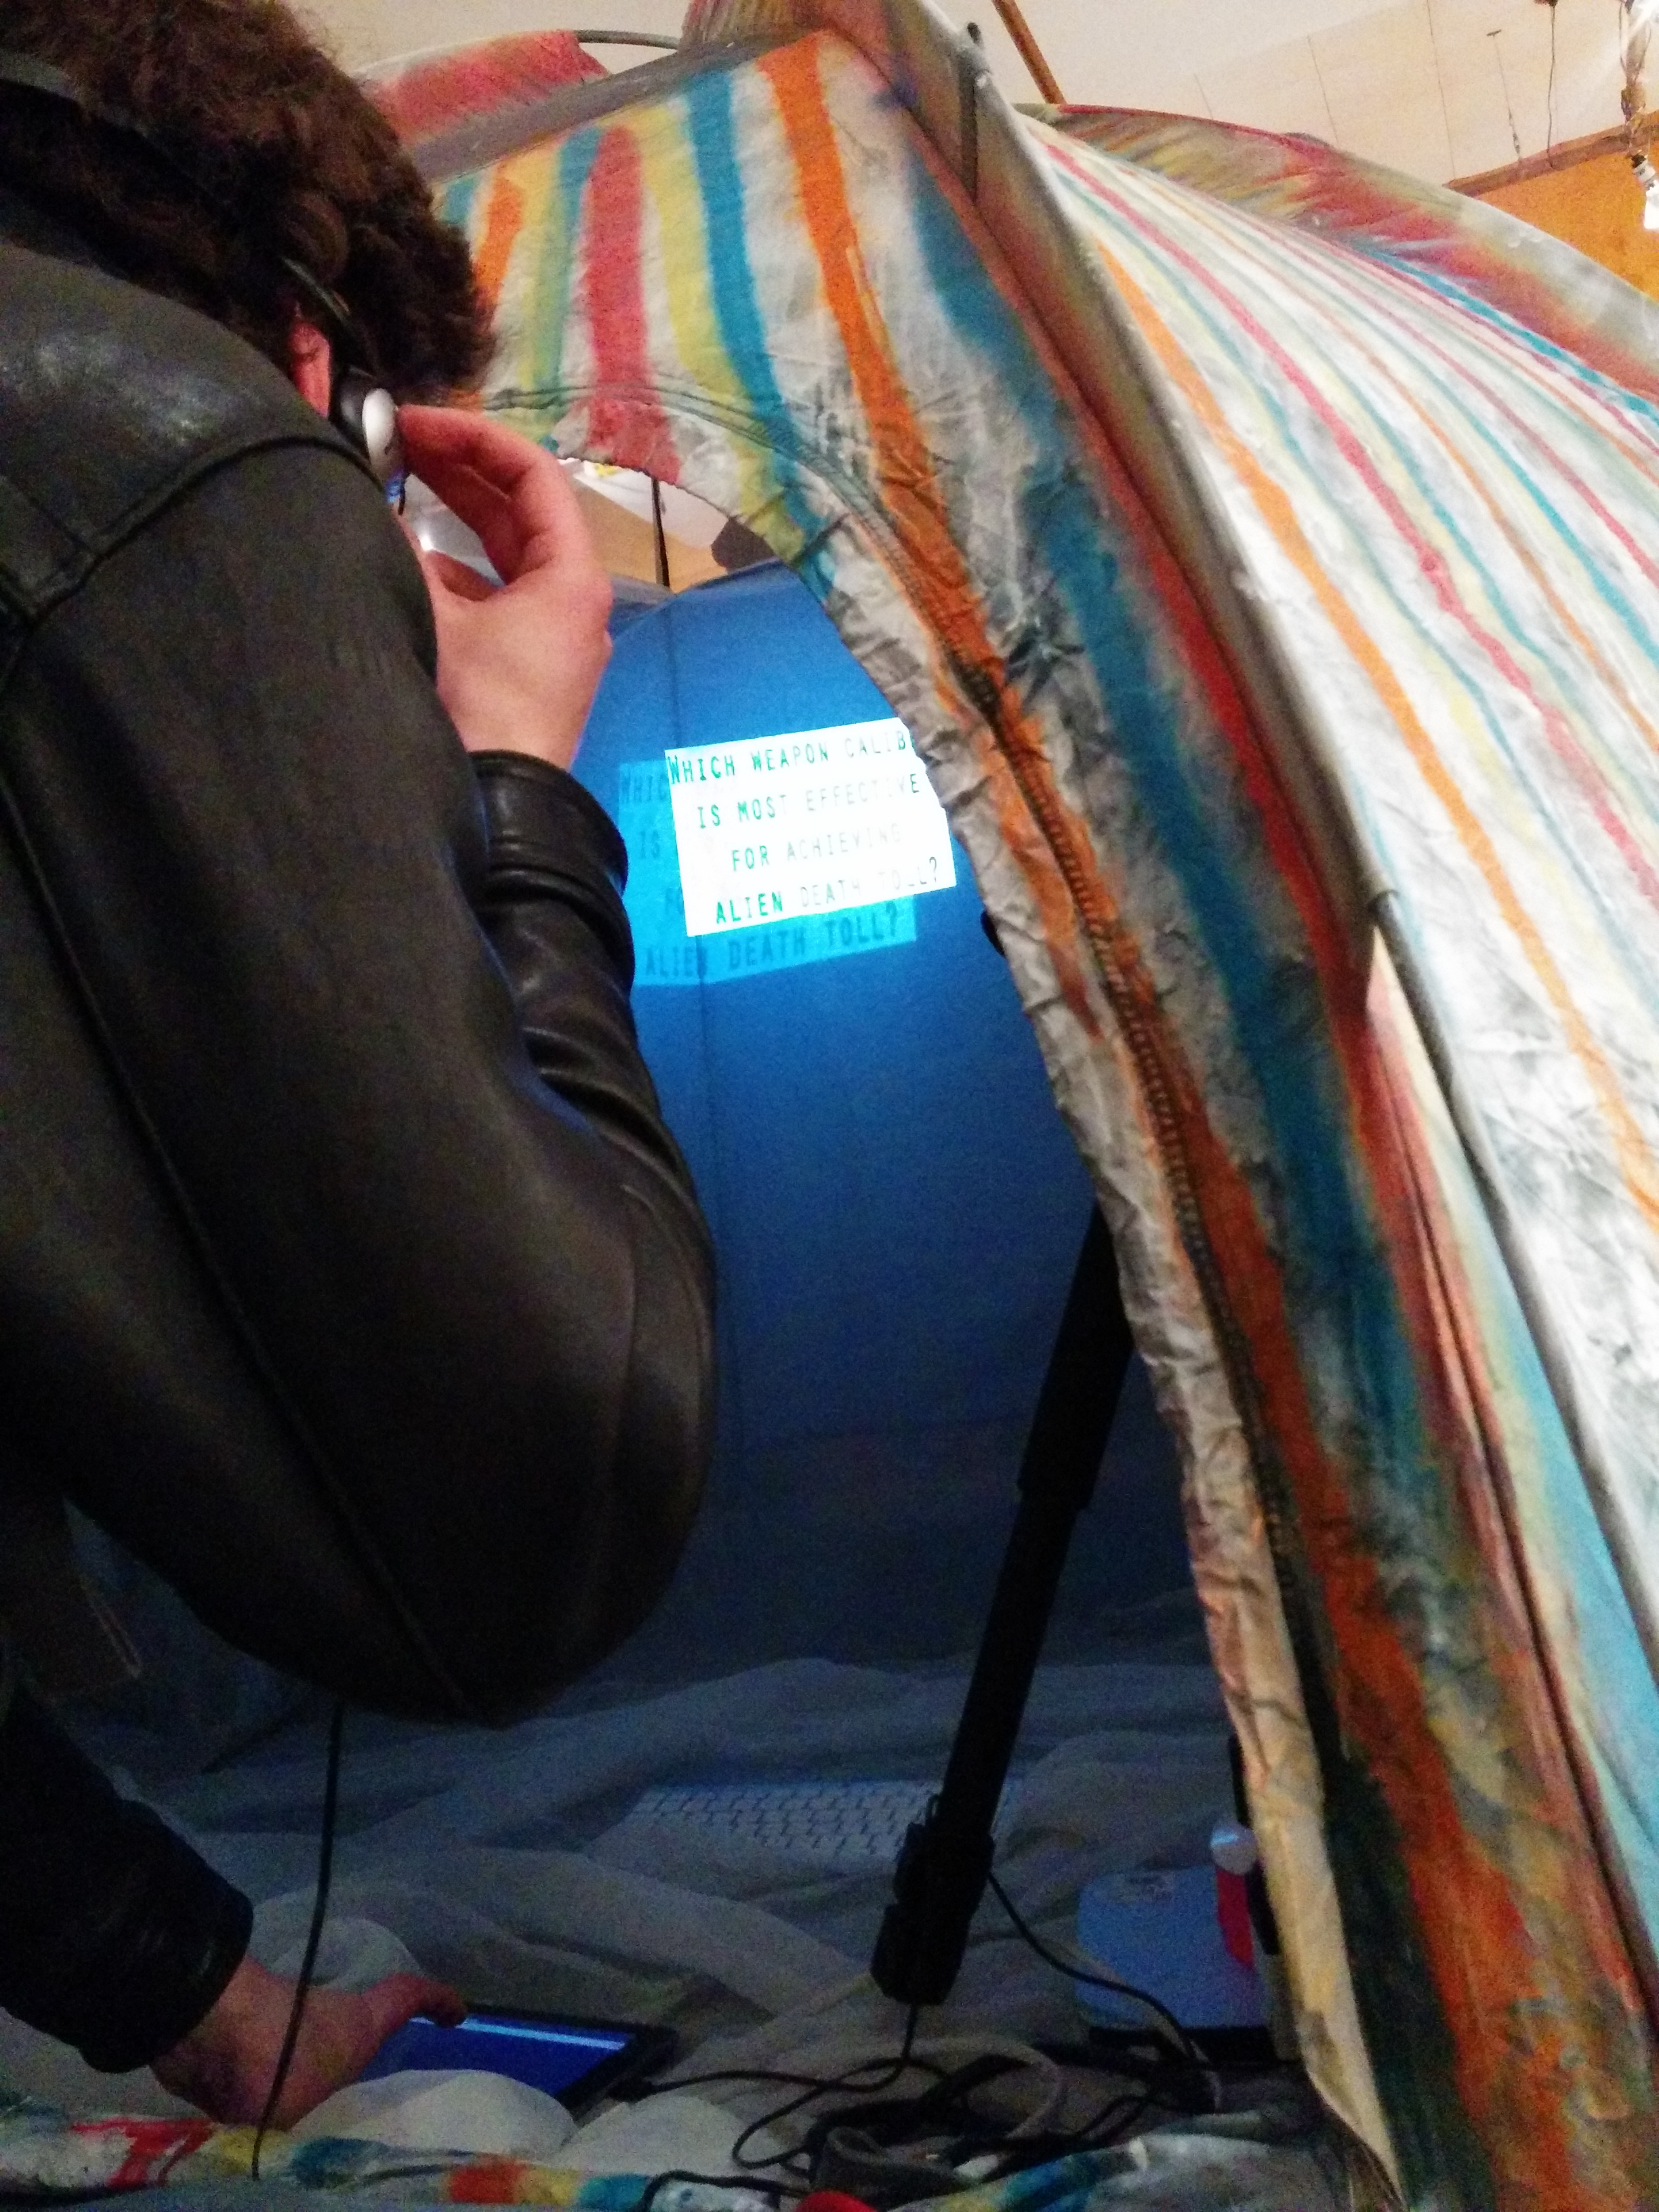
\includegraphics[width=0.7\textwidth]{psXXYborgTentPlay}
  \caption{Hannah Epstein\\psXXYborg at FAC 2014, playthrough view}
\end{figure}

\clearpage
\begin{figure}[!ht]
 \centering
  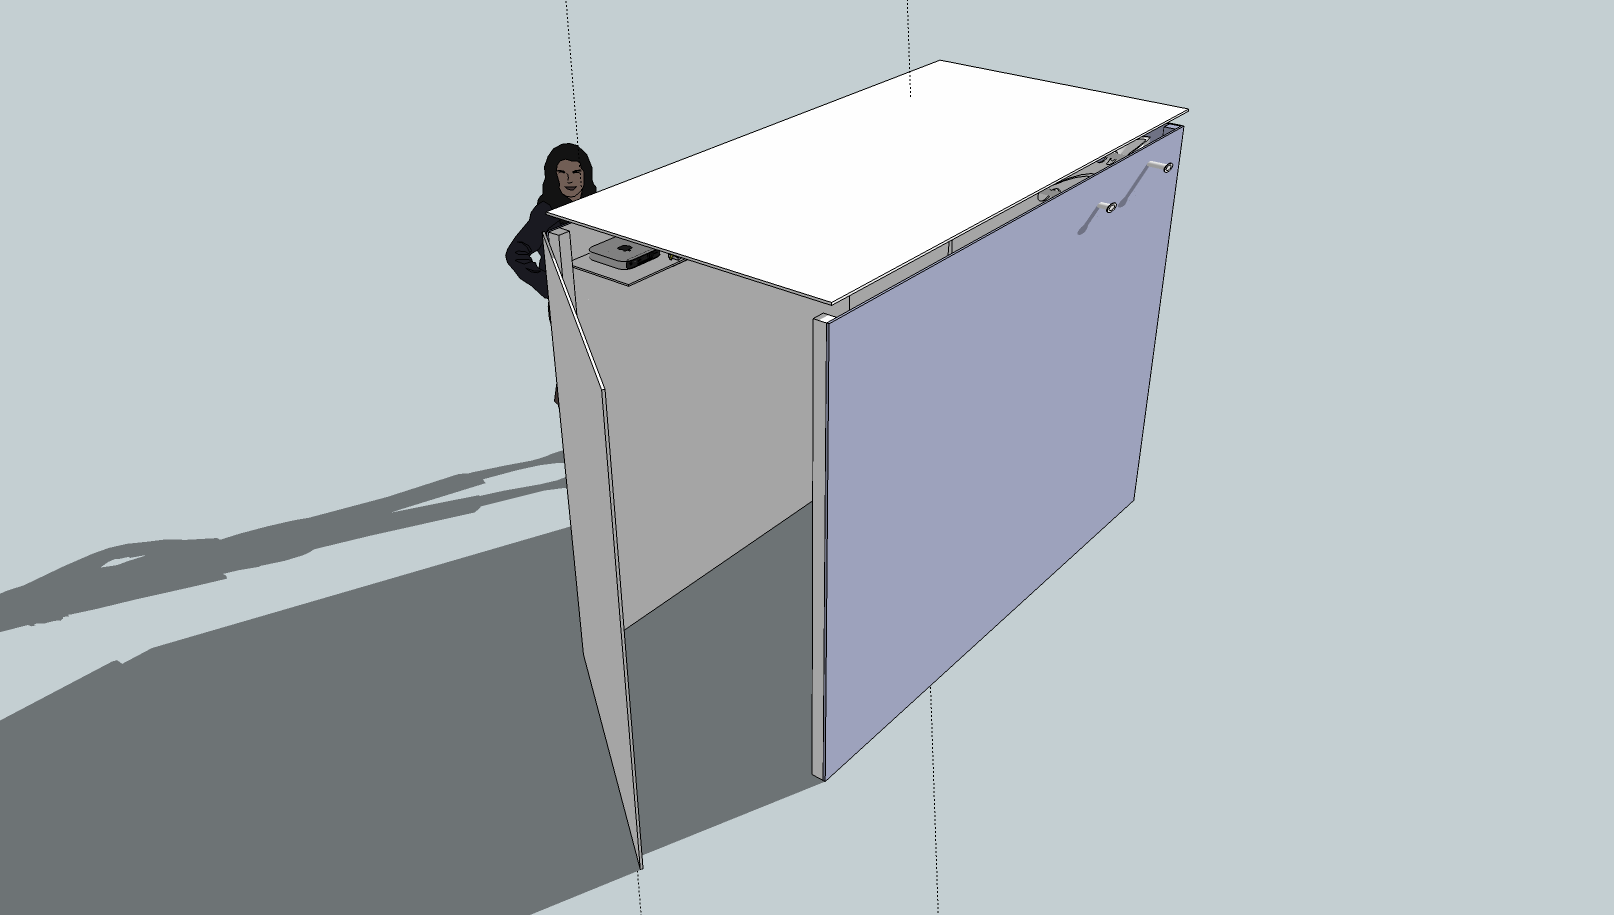
\includegraphics[width=\textwidth]{psXXYborgBox}
  \caption{Alex Leitch\\Concept for collapsible projection space 2013}
\end{figure}
\begin{figure}[!ht]
 \centering
  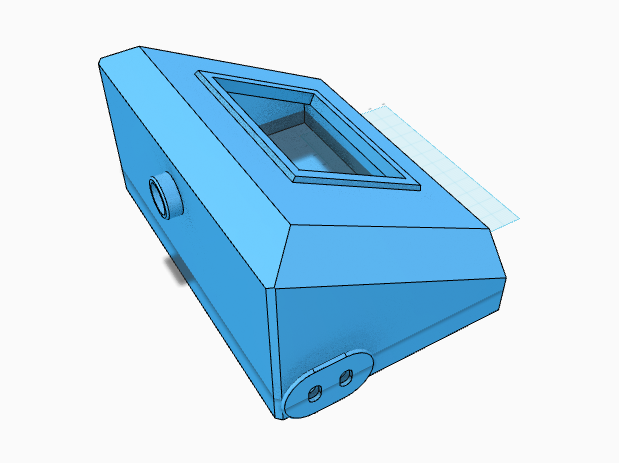
\includegraphics[width=\textwidth]{projectionBox}
  \caption{Alex Leitch\\Concept for portable arcade box, 2013}
\end{figure}

\clearpage

\section{Hardware Design}
The challenge of new media installations is huge. The success of a project like screenPerfect is dependent not only on its software, or on its ease of use, but on how straightforward it is to install on-site. The software is dependent on open wiFi and high bandwidth, a stable computing system, and a variety of computer interfaces. Idealistically, the software is open. In reality, it is incredibly difficult to build a new software system to work on broad platforms, and this ended up being an unrealistic goal.

Because the computing system needs to be stable and specfic, but does not need to be used for development, I began to look into appliance-appropriate hardware. There are a number of low-power ARM-controller based hardware platforms on the market at the time of writing, including the Arduino, the Beagle Bone, and the Raspberry Pi. All of these systems are designed to help artists make interactive works that take advantage of computing power for expression. The Arduino is a popular system for learning to build electronic interactions, the Beagle Bone a full-featured Linux computer, and the Raspberry Pi has come out of an idealistic foundation that hopes to encourage teenagers to learn to program and work with ultra-simplified computing systems.

The Raspberry Pi is my choice for building a system to support ScreenPerfect. It is simplified, plugs into a television set for a monitor, and uses a lightweight distribution of Debian linux as an operating system. Debian is famous because it has excellent package management. This means that when one installs software on Debian, the software tends to maintain its own dependencies, which reduces the amount of time a programmer spends adding and removing libraries to get something simple to work. Where an Arduino would require an entire secondary shield to access the internet, the Raspi is a full computer out of the box, able to access the internet while still being useful from the command line.

Raspberry Pi as a platform is also affordable, at \$35 for a Model B with ethernet port and 512Mb of RAM. Its operating system loads straight to an SD Card, which means it can be readily backed up and re-imaged should something happen to the hardware. In addition to this, the computer is the size of a credit card, which makes it straightforward to install in an artistic location such as a van or tent. The Raspberry Pi foundation is also a not-for-profit, which supports the opening of technical education to a broad range of children in the UK and overseas. This fit with the ideological stance of game::play Lab and the DMG, as well as my personal politics: that people should be able to use their tools as they see fit, and that technology should serve its users, rather than requiring the user to serve technology.

screenPerfect's technical display problems have been embedded in limited systems, such as a reliance on institutional wireless, designed to block filesharing, which also block peer-to-peer experiments such as screenPerfect's server from connecting to its client computers. This resulted in a need for a portable wireless hotspot to serve the application reliably, as in addition to blocking institutional routers, too many users would overwhelm the service. This provided a direction for my primary development to take: a computer that served both its own web application and provided its own infrastructure, from being turned on to when it was turned off, which did not require any kind of specialized setup for display. In addition, I began to consider how screenPerfect might exist in public space without the requirement of a "smart" screen or any kind of specialized interaction equipment.

People are willing to use their smartphones publicly, but mainly to access the external internet, or messaging services while they are in public. This led me to consider how people interact with the internet publicly, and to consider topics of privacy and public space, and how these problems have already been solved by galleries and coffee shops wishing to offer their clientele data services to promote engagement.

In public spaces, internet is supplied by wiFi, which comes through a specific type of router known as a "captive portal." A user will walk into a shop, attach to a network, and "sign" an agreement to make use of the wiFi within that space. 

Normally, the wiFi will then give them access to the external internet - the internet as supplied by a major ISP. The direction I have taken with the captive portal supplying itself with wiFi and a server was pioneered in 2013 by the Eyebeam project Subnod.es, in which users pair to a captive portal which is also a server, supplying access to an entirely private chat room, which is available only to users on the network supplied by the captive portal itself. 

The first issue addressed by this approach is that there is an inherent contradiction between downloading a site-specific piece to a personal device when the installed context is a core component of the aesthetic experience. Downloading applications to a smartphone seems invasive, particularly if those applications are experimental or site-specific, as - post-psXXYborg - I think that screenPerfect games are when they are at their best. The next is that web applications are very much not user specific - they can be experienced anywhere while they are on the open web, even if their content is intended to be restricted to a specific type of installation, or requires it for best use. 

A small, portable piece of resilient hardware seems to offer a solution. By serving the application locally, there is no reliance on an outside pipe. A copy of the game can be sold, customised, and stored in a collection, if such is desired, or installed in any kind of specific cabinet for later use. 

I decided on the Pi specifically because it is a cheap, accessible, reproducible system with a broad community of access and support, with the ability to include hardware controls where necessary. This type of system could also be built out on any leftover PC using a build of the Debian Linux system.

\section{Physical Deployment on the Raspberry Pi}
One of the earliest problems inherent to screenPerfect has been compromises in how the software is served to players and artists. Reliance on public internet is difficult, because the internet is not always available. WiFi is taken for granted in most institutions, but it is not always reliable, and the most interesting installation zones, such as the forest, may not have internet available at all. 

There are other challenges to public deployment, such as leaving a valuable production environment out in public, or requiring a technician to look in on specialized equipment. Both of these restrict the venues permitted for public display of work. Also limiting are instances where work should be deployed near people consuming alcohol, which is notoriously bad for electronics.

This chapter addresses my central response on how to reconcile the gap between an excellent idea for web-based deployment, and the physical reality of gallery spaces with sharply limited resources available for persistent software deployment. 


\newpage
\begin{figure}[h!]
 \centering
  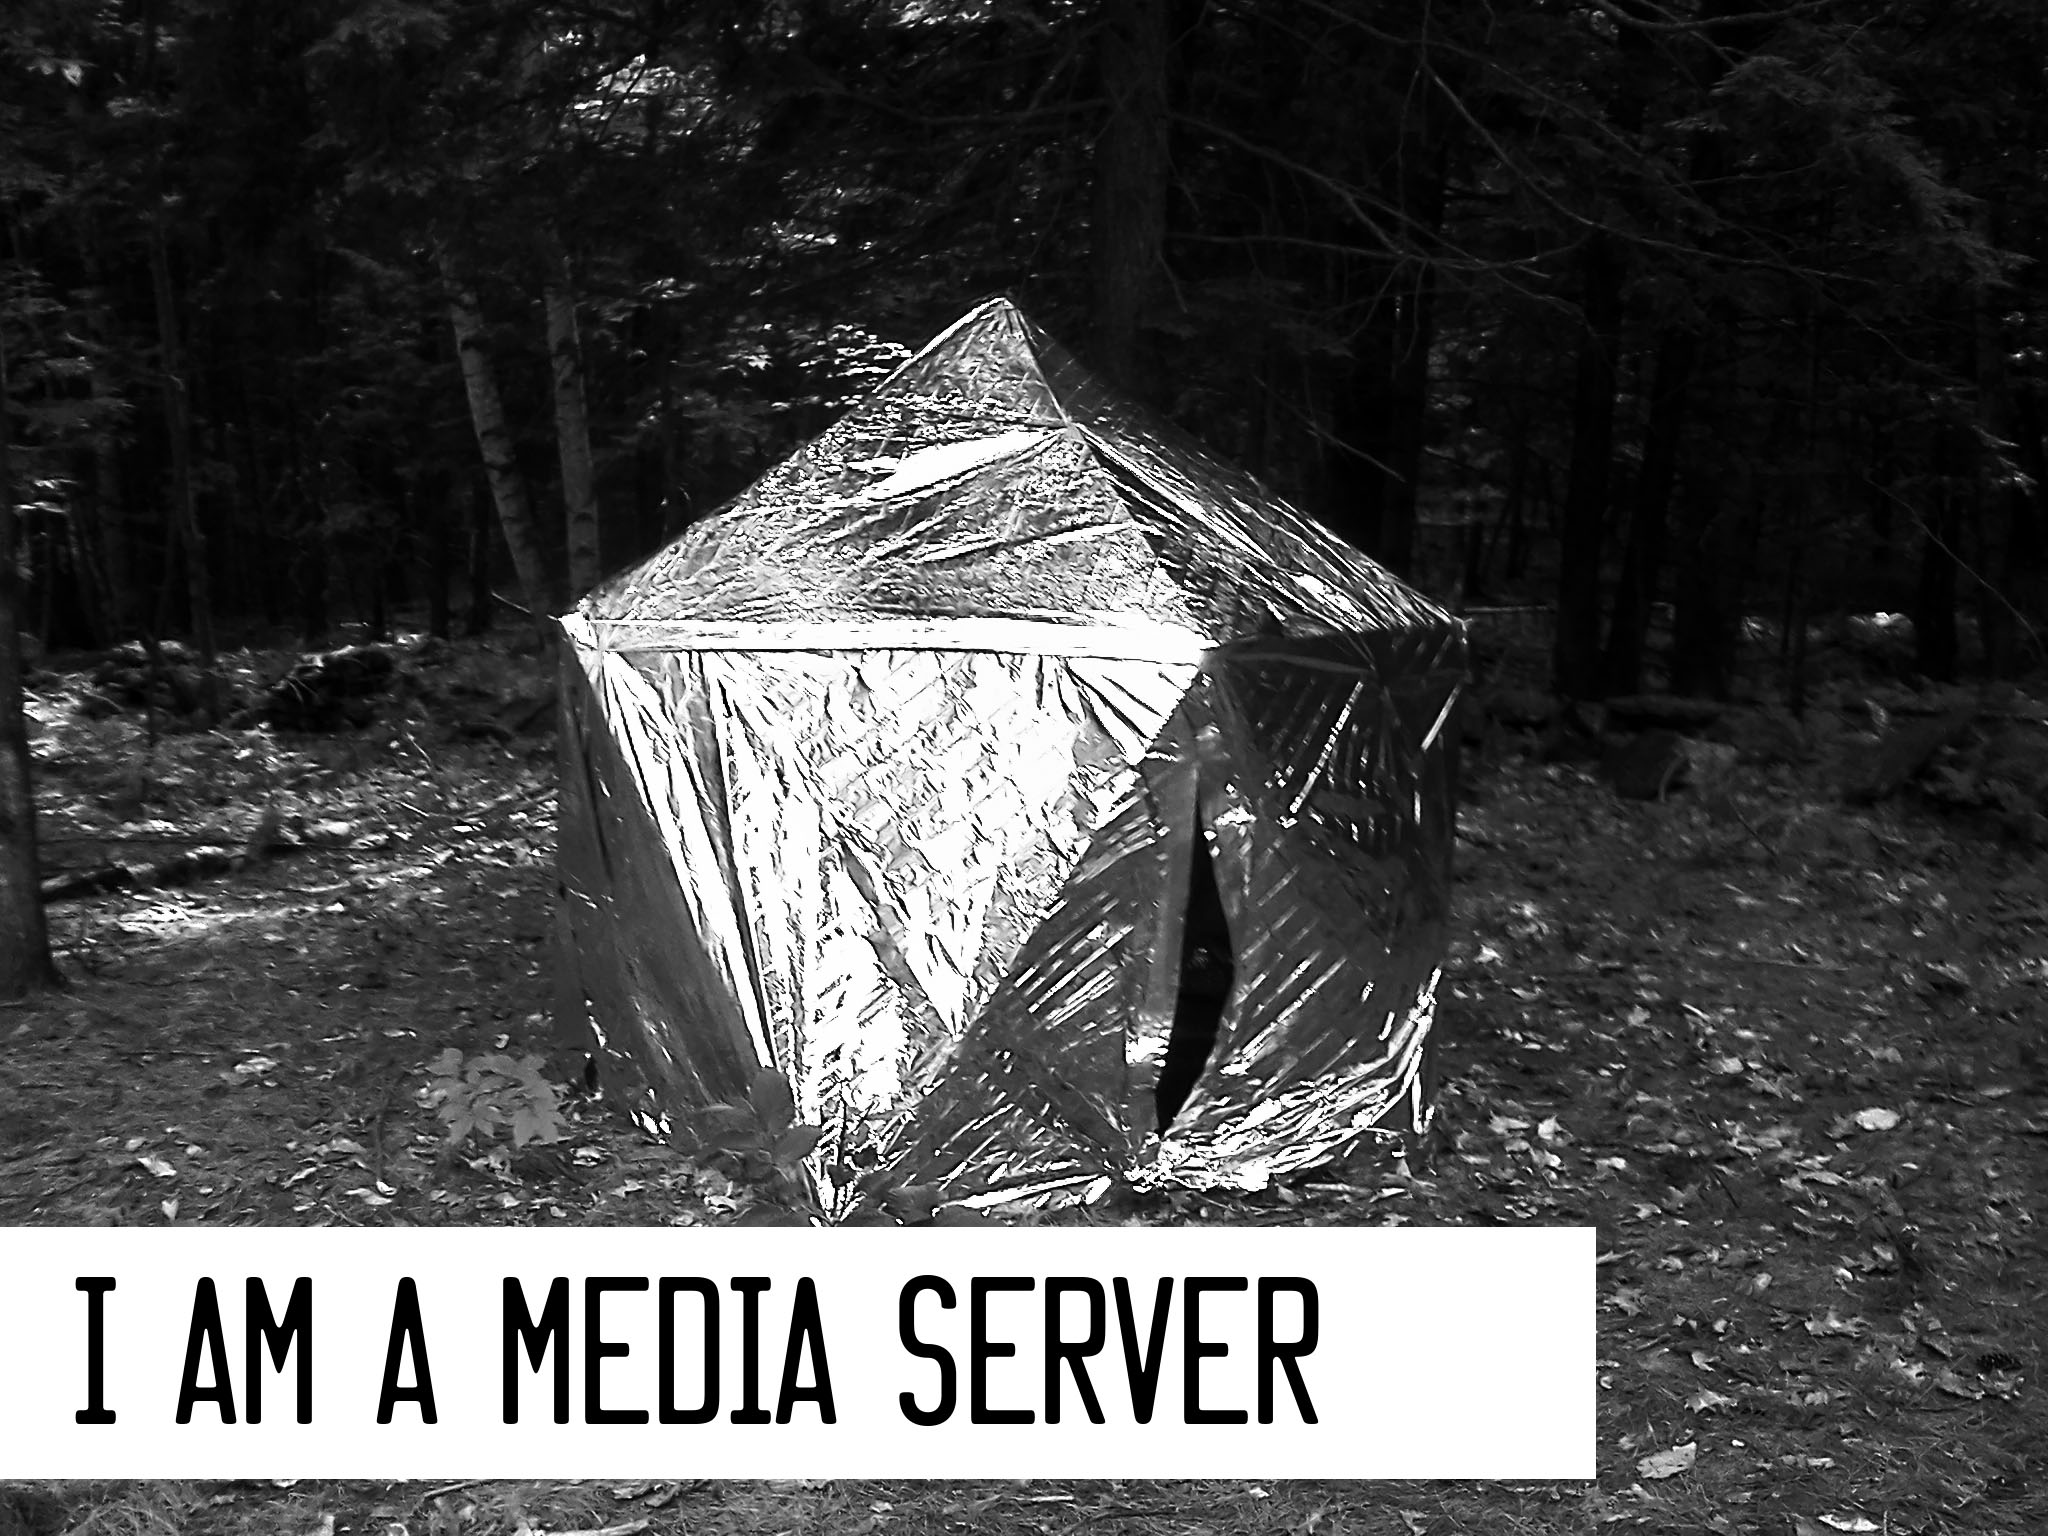
\includegraphics[width=\textwidth]{Seizuredome2}
  \caption{Abe Shulz and Sage Kochavi\\Seizuredome at FireFly 2013}
\end{figure}
\clearpage

\subsection{Problems and Complications in Display}
Some brainstorming resulted in the following scenarios that a reasonable arcade machine would need to address in order to present advanced work to the new, highly exclusive exhibit scenarios. 

\begin{enumerate}
\item Data service to an external source cannot be assumed to be available. 
\item The exhibit is assumed to be displayed in public
\item The environment is assumed to be meterologically hostile - hot or cold, wet or very dry, and to be hosting at least one party, such as an art opening, possibly with music
\item The exhibition is assumed to be supervised by technically untrained people.
\item The emphasis of the work should be on the work's display, rather than on a laptop screen.
\item The collectors of the work are assumed to have extremely limited resources for rugged workstations.
\item Any host-provided data carriage for external connection - wiFi - is assumed to be overloaded by default.
\end{enumerate}

 These are all very real constraints that impact display of new media art. We use computers for work and play, but we still separate our lives into periods when we pursue one or the other, and we still have boundaries between our personal and public lives. To use the same machines to display art as we do to build the work is to reduce the work from something approachable to any other tab in a computer. New media works especially must be seen within their exhibition context to be understood.

\subsection{Subnod.es and Public Private Space}
This project has a precursor using similar technology builtat Eyebeam in New York in 2013. Subnod.es uses a captive portal similar to my own, based on the inexpensive Raspberry Pi framework, to display a chat client to only the local environment. The differences are substantial, although mainly located within the code. Subnod.es relies on an external DNS being made available via the actual subnod.es software, and depends on a different collection of software to serve the portal proper. It is also built such that those library dependencies are inseparable from the main project script.

The chief concern of subnod.es I have not yet mentioned: subnod.es was built as a response to concerns about communications privacy in North America under the NSA. Specifically, the author is concerned that people behave differently when they are watched, a subset of the concerns generally associated with panoptica and totalitarianism. While I have not specifically structured screenPerfect's Art Portal to address these concerns, it has been built to be largely private. It serves an application to a limited selection of a public space.

The assumption of the Captive Portal Art Machine is that galleries have limited resources, but that people who go to art galleries almost certainly have access to a smart phone, which is a form of private space. Smart phones are people's own homes, and are built to assume that they will stay with their owners at all times. This means that to install an app is to ask a lot of a viewer: specifically, it is to ask someone to bring an application into their private space without getting to sample it first. To contrast, serving that same application on the broad internet is to entirely delimit the context the art may be experienced within, which reduces its scarcity value to almost nothing while simultaneously removing the curator's ability to set the context of an exhibition experience. This means that it's unlikely an artist can be compensated in any conventional sense, despite their large audience, and also means that the curation of the exhibit is no different than the "curation" found on Tumblr.

A better outcome might be to make a limited public space available in a private context, and this is what we are doing when we ask that people open their phones and look at a website. The Internet is, famously, the new public space. By presenting a web application using public technology within the exclusive context of the gallery - or desert, or forest - we take control again over how our art is presented, and from there, how it can be consumed. A gallery or exhibit space can be set up very specifically for the benefit of an audience in a way that the internet in general cannot be, and web technologies are uniform and affordable in the way that more custom projection design software is not.

This sense of limited private space is key to the code-switching that human communication relies on. We are not the same people in public as we are in private, and we are again different people when we are in different publics, work to the street to school to the gallery. Technology that sensitively addresses these different code contexts seems likely to benefit its authors and its users both, by permitting the integration of the personal focus with a personal device with the context of a semi-public facility or "safe space" for engagement with the art work.

\section{Distribution of Work}

This work has failed from the point of view of distribution at its conclusion. There is no reasonable way to distribute these works that is not reliant on a Node.JS enabled system being available, which means that ultimately, they are impossible to display as intended. I have included a record of the finished works built during No Jam 2 in my appendices, where they can be installed and played from disc, but they still require at minimum an installation of Node.JS to be played. Without that, they remain hidden. The point of this work is not the internet, so much as it is the possibilities present in the technology we rely upon for the internet to be accessible.

In the meantime, I have built individual variants of finished game jam games and shipped them in complete SD cards to their owners, so that, with a little effort, they can be run from any Model B Raspberry Pi just like a game cartridge.